%-------------------------------------------------
%% Única:
%-------------------------------------------------
\section{Características}
\label{sec:caracteristicas}

\subsection*{Única}
\begin{frame}{O que torna uma coisa única?}
	
	\begin{figure}[H]
		
\includegraphics[width=.5\textwidth]{ip.png}\footnotemark
	\end{figure}
	
	\footnotetext{http://www.multipetros.gr/posts/tag/ip/}
\end{frame}

%-------------------------------------------------
%% Análise:
%-------------------------------------------------
\subsection*{Análise}
\begin{frame}{Como analisar os dados?}
	\begin{block}{}
		\textbf{Pessoas} são ruins em captar e analisar dados. \\Motivos: tempo, precisão e regularidade.
	\end{block}
	
	\begin{itemize}
		\item \textit{Big Data} - Processamento de alta peformance;
		\item Inteligência Artificial: 
		\begin{itemize}
			\item Redes neurais; 
			\item Algoritmos Genéticos;
			\item Lógica \textit{Fuzzy}...
		\end{itemize}
	\end{itemize}
	
	\begin{figure}[H]
		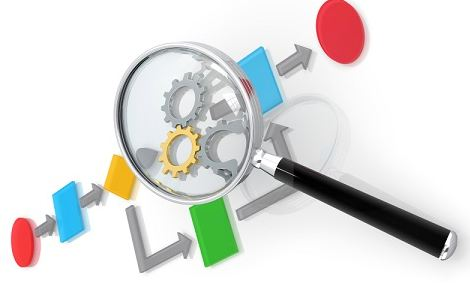
\includegraphics[width=.4\textwidth]{analise.jpg}\footnotemark
	\end{figure}
	
	\footnotetext{http://www.bankers-adda.com/wp-content/uploads/2015/11/}
\end{frame}

%-------------------------------------------------
%% Comunicação:
%-------------------------------------------------
\subsection*{Comunicação}
\begin{frame}{Como as coisas se falam?}
	\begin{block}{Sensores}
		\begin{itemize}
			\item Térmicos; Vibração; Presença; Som; Pressão; Lumisosidade; Fumaça...
		\end{itemize}
	\end{block}
	
	\begin{columns}
		\column{0.4\linewidth}
		\begin{block}{Protocolos}
			\begin{itemize}
				\item MQTT:
					\begin{itemize}
						\item \textit{Publish/Subscribe};
						\item M2M;
						\item TCP/IP.
					\end{itemize} 
				\item HTTP: 
					\begin{itemize}
						\item \textit{Client/Server};
						\item Bidirecional;
						\item TCP/IP.
					\end{itemize}
			\end{itemize}
		\end{block}
		
		\column{0.5\linewidth}
		\begin{block}{Conectividade}
			\begin{itemize}
				\item 2G - Mensagens;
				\item 3G - Áudio e Vídeo;
				\item 4G - Sem distinção, é tudo dado;
				\item 5G - Tudo dado, mas com baixa latência e alta velocidade.
			\end{itemize}
		\end{block}
	\end{columns}
\end{frame}

\begin{frame}{Arquitetura}
	\begin{figure}[H]
		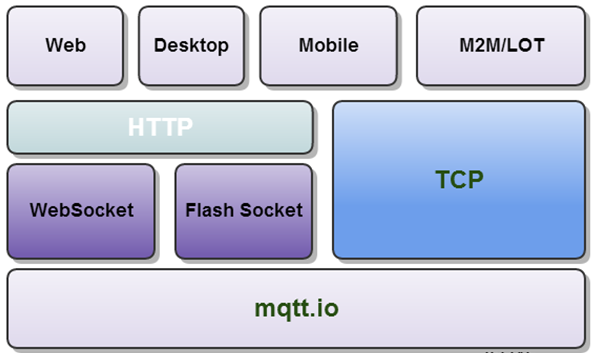
\includegraphics[width=.9\textwidth]{comunicacao.png}\footnotemark
	\end{figure}
	
	\footnotetext{http://images.cnitblog.com/blog/120296/201406/}
\end{frame}

%-------------------------------------------------
%% Controle:
%-------------------------------------------------
\subsection*{Controle}
\begin{frame}{Como controlar a aplicação?}
	\begin{itemize}
		\item A qualquer hora;
		\item De qualquer lugar.
	\end{itemize}
	
		\begin{figure}[H]
			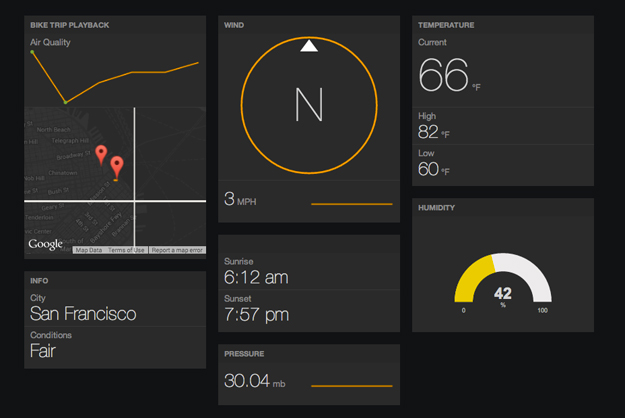
\includegraphics[width=.6\textwidth]{controle.jpg}\footnotemark
		\end{figure}
		
		\footnotetext{https://cdn.psfk.com/wp-content/uploads/2014/05/}
\end{frame}

%-------------------------------------------------
%% Estrutura:
%-------------------------------------------------
\section{Estrutura}
\label{sec:estrutura}

\subsection*{Integração}
\begin{frame}{Multidisciplinariedade}
	\begin{columns}
		\column{0.3\linewidth}
		\begin{itemize}
			\item Eletrônica;
			\item Robótica;
			\item Mecânica;
			\item Computação.
		\end{itemize}
		
		\column{0.7\linewidth}
		\begin{figure}[H]
			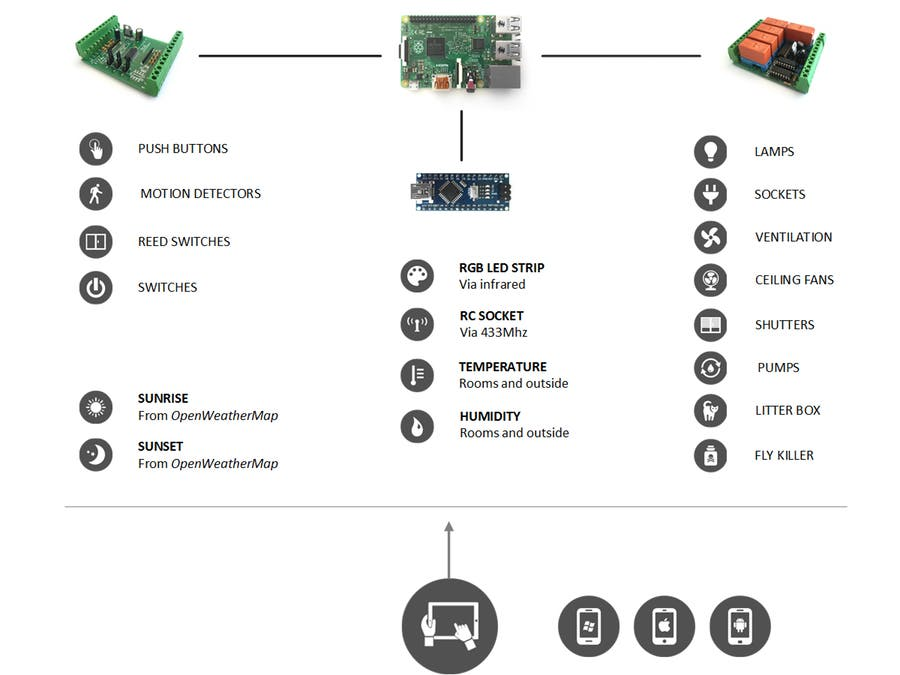
\includegraphics[width=1\textwidth]{multi.jpg}\footnotemark
		\end{figure}
	\end{columns}
	\footnotetext{https://hackster.imgix.net/uploads/cover\_image/file/81451/}
\end{frame}

%-------------------------------------------------
%% Hardware:
%-------------------------------------------------
\subsection*{Hardware}
\begin{frame}{Raspberry Pi}
	\begin{figure}[H]
		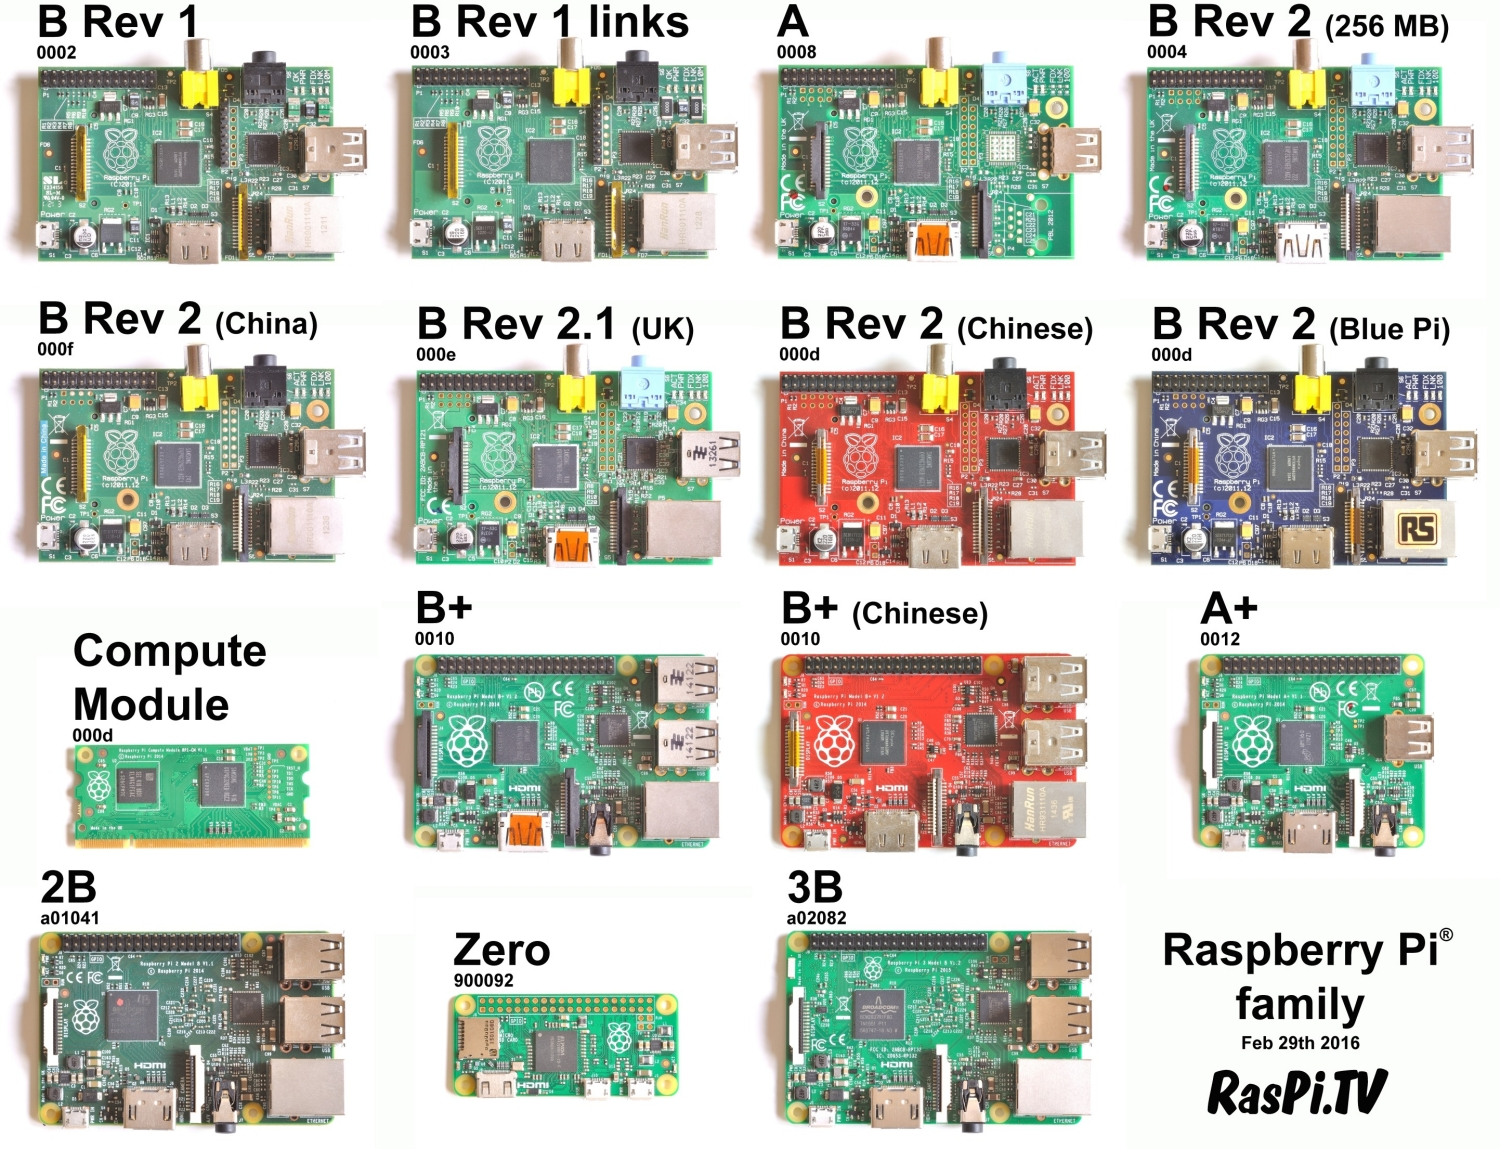
\includegraphics[width=.7\textwidth]{raspberryfamily.jpg}\footnotemark
	\end{figure}
	
	\footnotetext{http://raspi.tv/2016/raspberry-pi-family-photo-updated-to-include-pi3b-29-feb-2016}
\end{frame}

\begin{frame}{Arduino}
	\begin{figure}[H]
		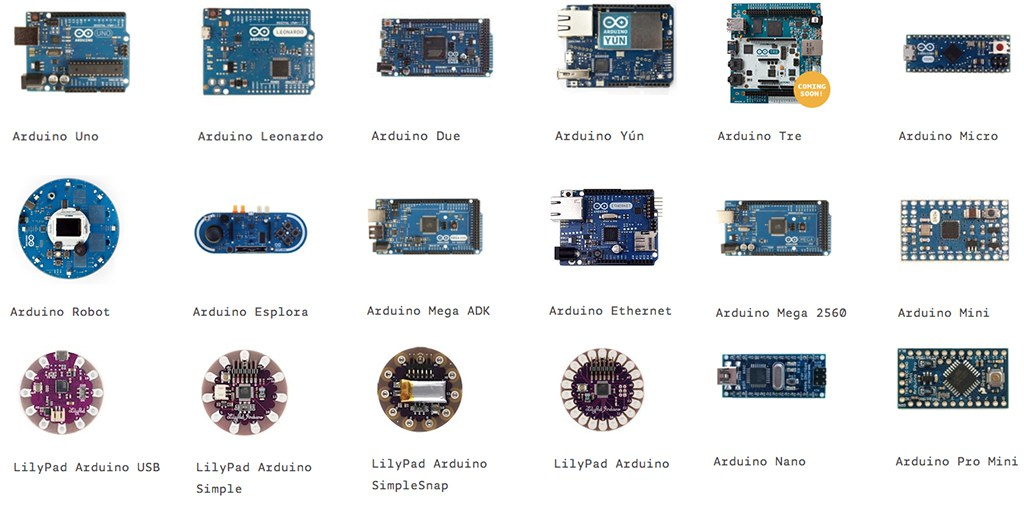
\includegraphics[width=1\textwidth]{arduinofamily.jpg}\footnotemark
	\end{figure}
	
	\footnotetext{https://i1.wp.com/electronicshacking.com/wp-content/uploads/2016/05/}
\end{frame}

\begin{frame}{ESP8266}
	\begin{figure}[H]
		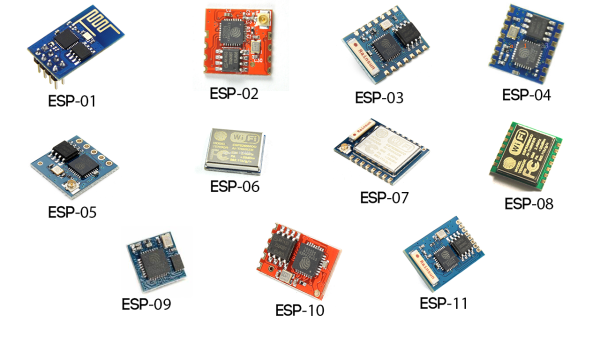
\includegraphics[width=.9\textwidth]{espfamily.png}\footnotemark
	\end{figure}
	
	\footnotetext{https://qph.ec.quoracdn.net/main-qimg-722e4cace72b92ca0efce373866d08c2}
\end{frame}

\begin{frame}{Módulo Relé}
	\begin{figure}[H]
		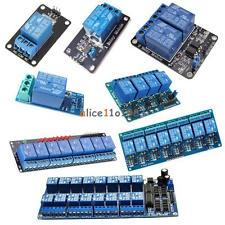
\includegraphics[width=.5\textwidth]{relayfamily.jpg}\footnotemark
	\end{figure}
	
	\footnotetext{http://thumbs.ebaystatic.com/images/m/mzkfWblEtqpHZfTceI9Bh9A/}
\end{frame}

%-------------------------------------------------
%% Software:
%-------------------------------------------------
\subsection*{Software}
\begin{frame}{}
	\begin{block}{Principais linguagens}
		\begin{itemize}
			\item Java;
			\item C/C++;
			\item Lua;
			\item Python;
			\item JavaScript;
			\item PHP.
		\end{itemize}
	\end{block}
\end{frame}

%-------------------------------------------------
%% Problemas:
%-------------------------------------------------
\section{Problemas}

\subsection*{Endereçamento}
\begin{frame}{}
	\begin{figure}[H]
		
\includegraphics[width=1\textwidth]{ipv4_stock.jpg}\footnotemark
	\end{figure}
	
	\footnotetext{https://victorh2007.files.wordpress.com/2014/06/}
\end{frame}

\subsection*{Segurança}
\begin{frame}{}
	\begin{block}{\cite{ComputerWorld}}
		\begin{itemize}
			\item Com tantas coisas conectadas à web, os institutos de pesquisa apontam aspectos negativos em relação à segurança. Eles indicam que dentro de \textbf{dois anos}, 90\% de todas as redes de TI terão uma falha de segurança derivada da IoT.
			\item Em 2013, hackers americanos invadiram um carro conectando-se à porta serial do veículo. Esse tipo de conexão é comumente utilizada para análise e manutenção dos veículos.
			\item Em 2015, eles repetiram o ataque via \textit{wireless}.
		\end{itemize}
	\end{block}
\end{frame}

\subsection*{Privacidade}
\begin{frame}{}
	\begin{block}{\cite{PedroValente} e \cite{P2413}}
		\begin{itemize}
			\item Proteção de dados pessoais;
			\item Hábitos, localização, interesses e preferências pessoais;
			\item Fluxo constante de informação;
			\item Normalização dos sistemas inteligentes.
		\end{itemize}
	\end{block}
\end{frame}

%-------------------------------------------------
%% Como começar:
%-------------------------------------------------
\section{Por onde começar?}
\label{sec:comeco}

\subsection*{Pesquise}
\begin{frame}{}
	\begin{block}{\textit{Links} para leitura (nas referências)}
		\begin{itemize}
			\item Windows 10 IoT \cite{WindowsIot};
			\item Intel IoT \cite{IntelIot};
			\item Raspberry and Google IoT Project \cite{RaspberryGoogleIot};
			\item Arduino IoT \cite{ArduinoIot}.		
		\end{itemize}
	\end{block}
\end{frame}

\subsection*{Faça Você Mesmo!}
\begin{frame}{}
	\begin{block}{\textit{Links} para praticar (nas referências)}
		\textbf{Pré-requisito: Inglês básico}
		\begin{itemize}
			\item Dweet.io - A rede social das máquinas \cite{DweetIot};
			\item ThingSpeak - Análise de dados \cite{ThingSpeakIot};
			\item Highcharts - Análise de dados e gráficos \cite{HighChartsIot};
			\item FreeBoard - Controle das coisas \cite{FreeBoardIot};
			\item Instructables - Ideias pra replicar (Básico) \cite{InstructablesIot}. 
			\item Hackaday - Ideias pra replicar (Avançado) \cite{InstructablesIot}.
		\end{itemize}
	\end{block}
	\begin{figure}[H]
		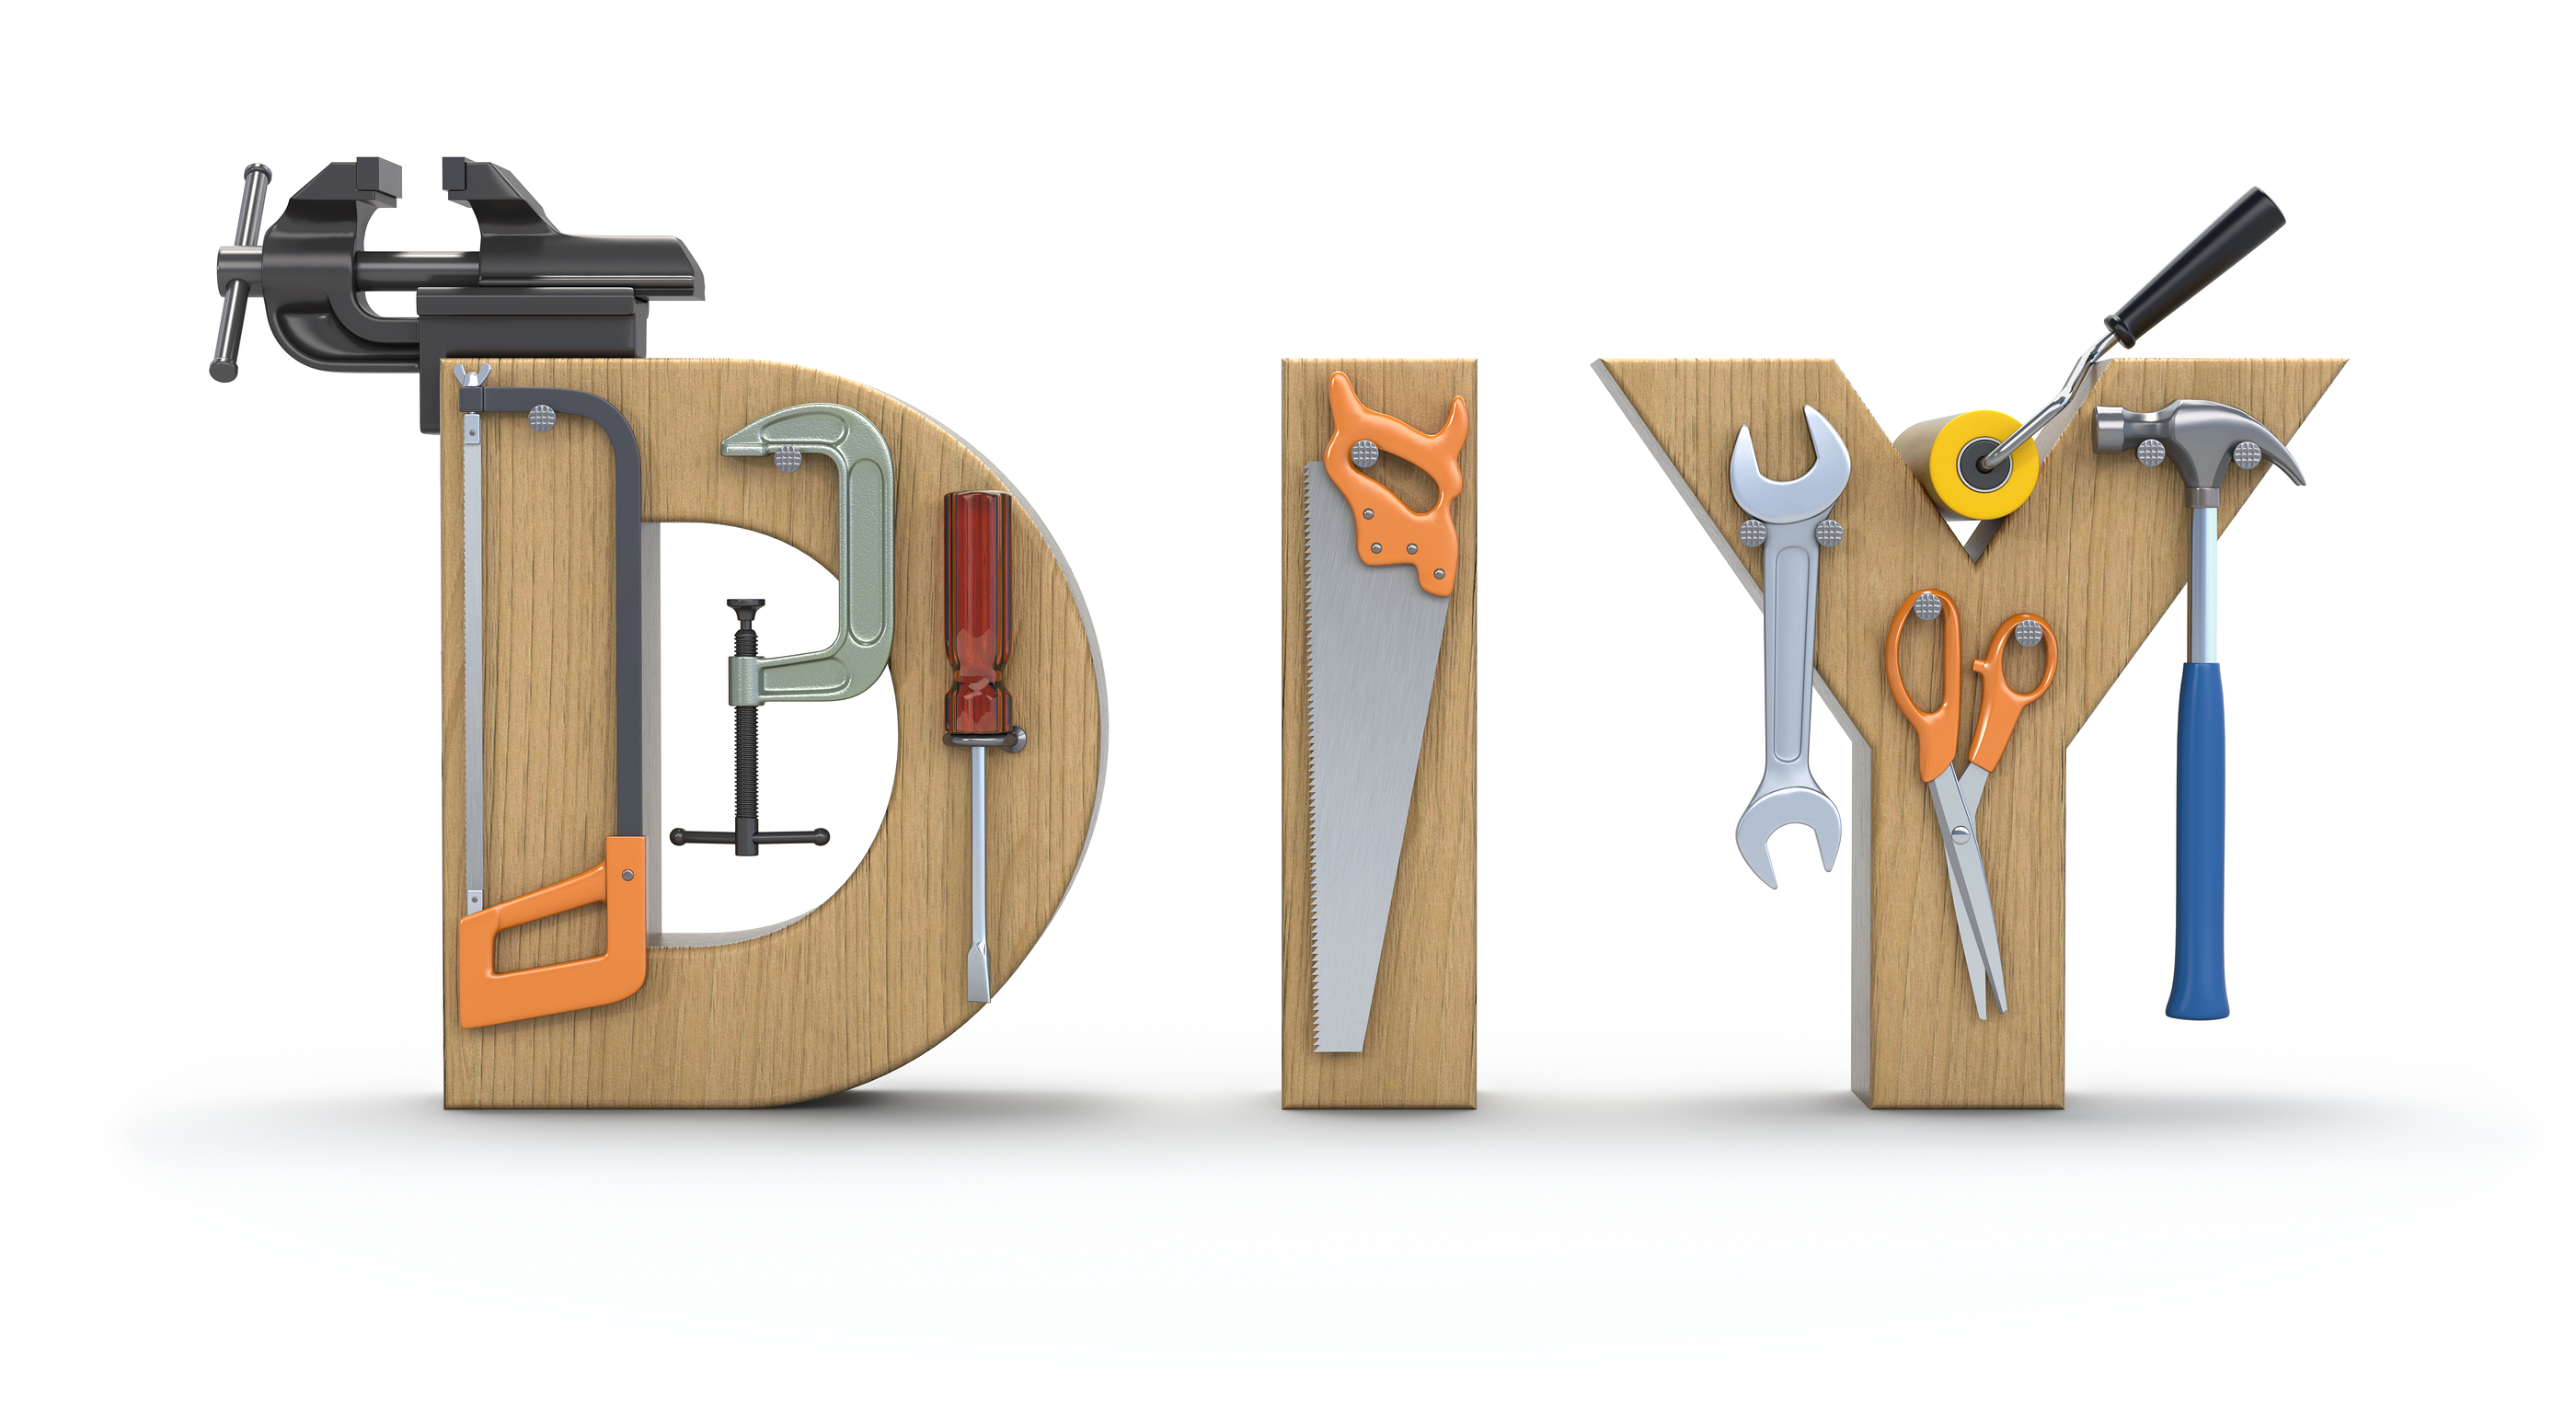
\includegraphics[width=.5\textwidth]{diy.jpg}\footnotemark
	\end{figure}
	
	\footnotetext{http://mydogsjournal.com/wp-content/uploads/2013/12/}
\end{frame}